% title: Output and path weight are separate channels
% description: The program returns its original output. Each reached factor multiplies a path weight initialized to one, so factors a and b contribute a times b.
\documentclass[tikz,border=5pt]{standalone}
\usetikzlibrary{arrows.meta,calc,shapes.geometric}
\definecolor{numeric}{HTML}{4477AA}
\definecolor{textual}{HTML}{AA4499}

\tikzset{
    box/.style={draw, line width=0.8pt, minimum height=0.8cm,
                minimum width=1.8cm, inner sep=6pt, align=center},
    ir/.style={box},
    flow/.style={-{Stealth[length=5pt]}, line width=0.9pt},
    feedback/.style={flow, dashed},
    note/.style={font=\small, align=center},
    choice/.style={diamond, draw, line width=0.8pt,
                   aspect=2, inner sep=2pt, align=center},
}

\newcommand{\irframe}[2]{
    \draw[line width=0.8pt] #1 rectangle #2;
}

\newcommand{\transformarrow}[4][above]{
    \draw[flow] (#2) -- node[#1=6pt,note] {#4} (#3);
}

\begin{document}
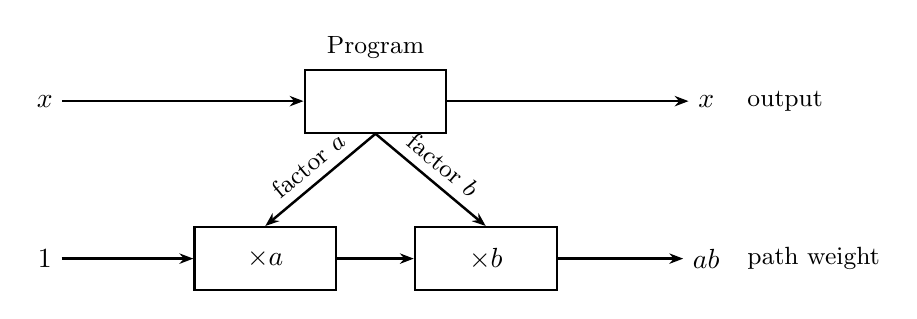
\begin{tikzpicture}

    \node (x) at (0,1) {$x$};
    \node[ir, label={[note]above:Program}] (program) at (4.2,1) {};
    \node (out) at (8.4,1) {$x$};
    \draw[flow] (x) -- (program);
    \draw[flow] (program) -- (out);
    \node[note,anchor=west] at (8.8,1) {output};
    \node (one) at (0,-1) {$1$};
    \node[box] (a) at (2.8,-1) {$\times a$};
    \node[box] (b) at (5.6,-1) {$\times b$};
    \node (weight) at (8.4,-1) {$ab$};
    \draw[flow] (one) -- (a);
    \draw[flow] (a) -- (b);
    \draw[flow] (b) -- (weight);
    \draw[flow] (program.south) -- node[above,sloped,note] {factor $a$} (a.north);
    \draw[flow] (program.south) -- node[above,sloped,note] {factor $b$} (b.north);
    \node[note,anchor=west] at (8.8,-1) {path weight};

\end{tikzpicture}
\end{document}
